%!TEX root = thesis.tex
%=============================================================================


\chapter{Evaluation}

In this chapter two tests will be presented which were used to evaluate the proposed speech recognition pipeline.

\section{Robocup Speech Recognition Test}


\begin{figure}[ht]	
	\centering
	\subfloat[Scenario for baseline of proposed pipeline]{
		
\includegraphics[width=0.5\textwidth]{diagrams/robocup_task_t.pdf}
	}
	\subfloat[Scenario for elongated baseline of proposed pipeline]{
		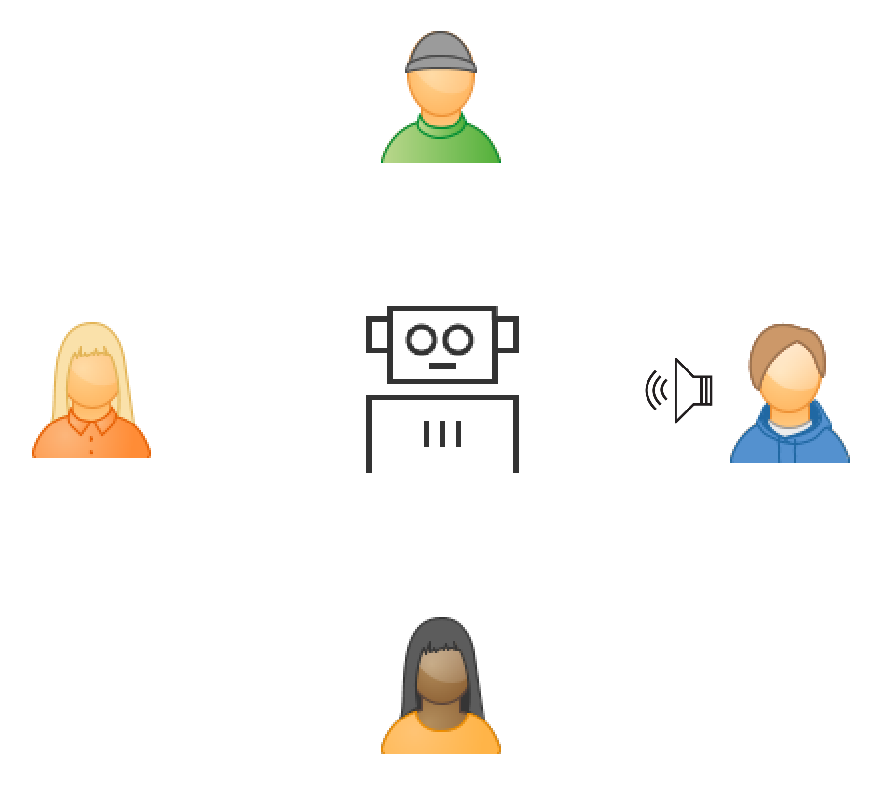
\includegraphics[width=0.5\textwidth]{diagrams/robocup_task_t1.pdf}
	}
	
	\caption{Test scenario for the RoboCup task}
	\label{pic:eval_task}
\end{figure}

\begin{figure}[ht]
	\begin{tabular}{ | l | l | l | l |}
		\hline
		Run & Correctly recognized sentences & Points & Points by SSL \\ \hline
		1 & 50\% & 45 & 0 \\ \hline
		2 & 50\% & 40 & 10 \\ \hline
		4 & 35\% & 25 &  0 \\ \hline
		5 & 40\% & 30 & 10 \\ \hline
		6 & 45\% & 40 & 10 \\ \hline
		7 & 60\% & 50 & 10 \\ \hhline{|=|=|=|=|} 
		Avg & 46.7\% & 38.3 & 6.7 \\
		\hline
	\end{tabular}
	\caption{Results of the existing pipeline in the RoboCup task}
	\label{pic:eval_task_results_old}
\end{figure}

\begin{figure}[ht]
	\begin{tabular}{ | l | l | l | l |}
		\hline
		Run & Correctly recognized sentences & Points & Points by SSL \\ \hline
		1 & 65\% & 50 &  0 \\ \hline
		2 & 55\% & 70 & 20 \\ \hline
		4 & 55\% & 35 &  0 \\ \hline
		5 & 55\% & 50 & 20 \\ \hline
		6 & 60\% & 60 &  0 \\ \hline
		7 & 60\% & 60 & 10 \\ \hhline{|=|=|=|=|} 
		Avg & 58.3\% & 54.2 & 8.3\\
		\hline
	\end{tabular}
	\caption{Results of the proposed pipeline in the RoboCup task}
	\label{pic:eval_task_results_new}
\end{figure}

\begin{itemize}
	\item oftentimes recognition results would be very similar, but once wrong and once right, e.g. ''whats the color of the coke'' would be once interpreted by both pipelines as ''whats the color of the bowl'' and once by the old pipeline as ''whats the color of the fork'' and once correct by the proposed pipeline; other example: sponge was recognized as sausages, thus once wrong
\end{itemize}


%----------------------------------------------------------------------------------------------------


\section{Dataset Evaluation}

\begin{figure}[ht]
	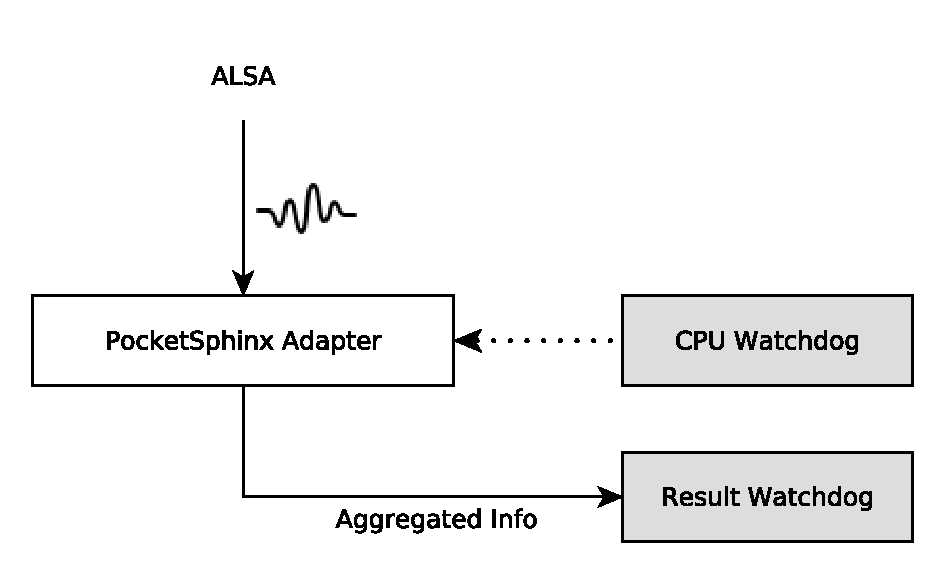
\includegraphics[width=0.66\textwidth]{diagrams/eval_pipeline_1.pdf}
	\caption{Test scenario for existing pipeline}
	\label{pic:eval_p1_diag}
\end{figure}

\begin{figure}[ht]	
	\centering
	\subfloat[Scenario for baseline of proposed pipeline]{
		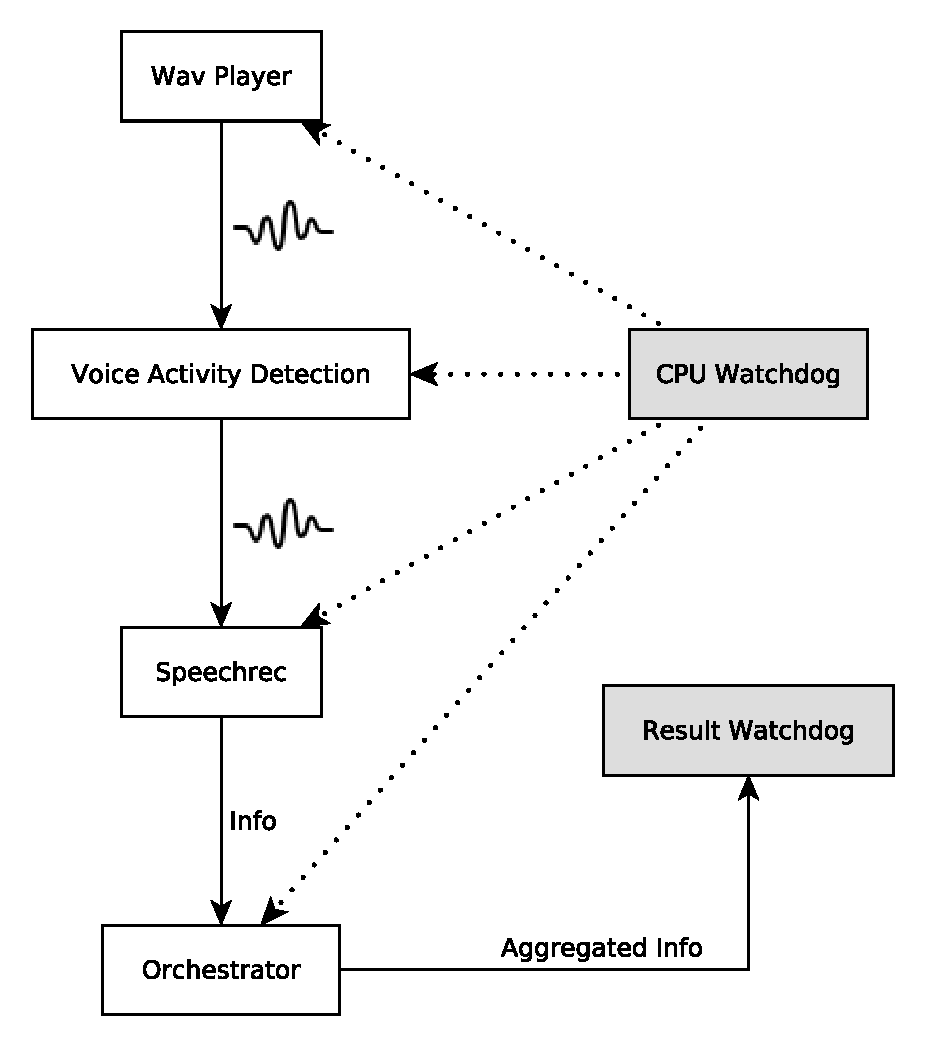
\includegraphics[width=0.5\textwidth]{diagrams/eval_pipeline_2.pdf}
	}
	\subfloat[Scenario for elongated baseline of proposed pipeline]{
		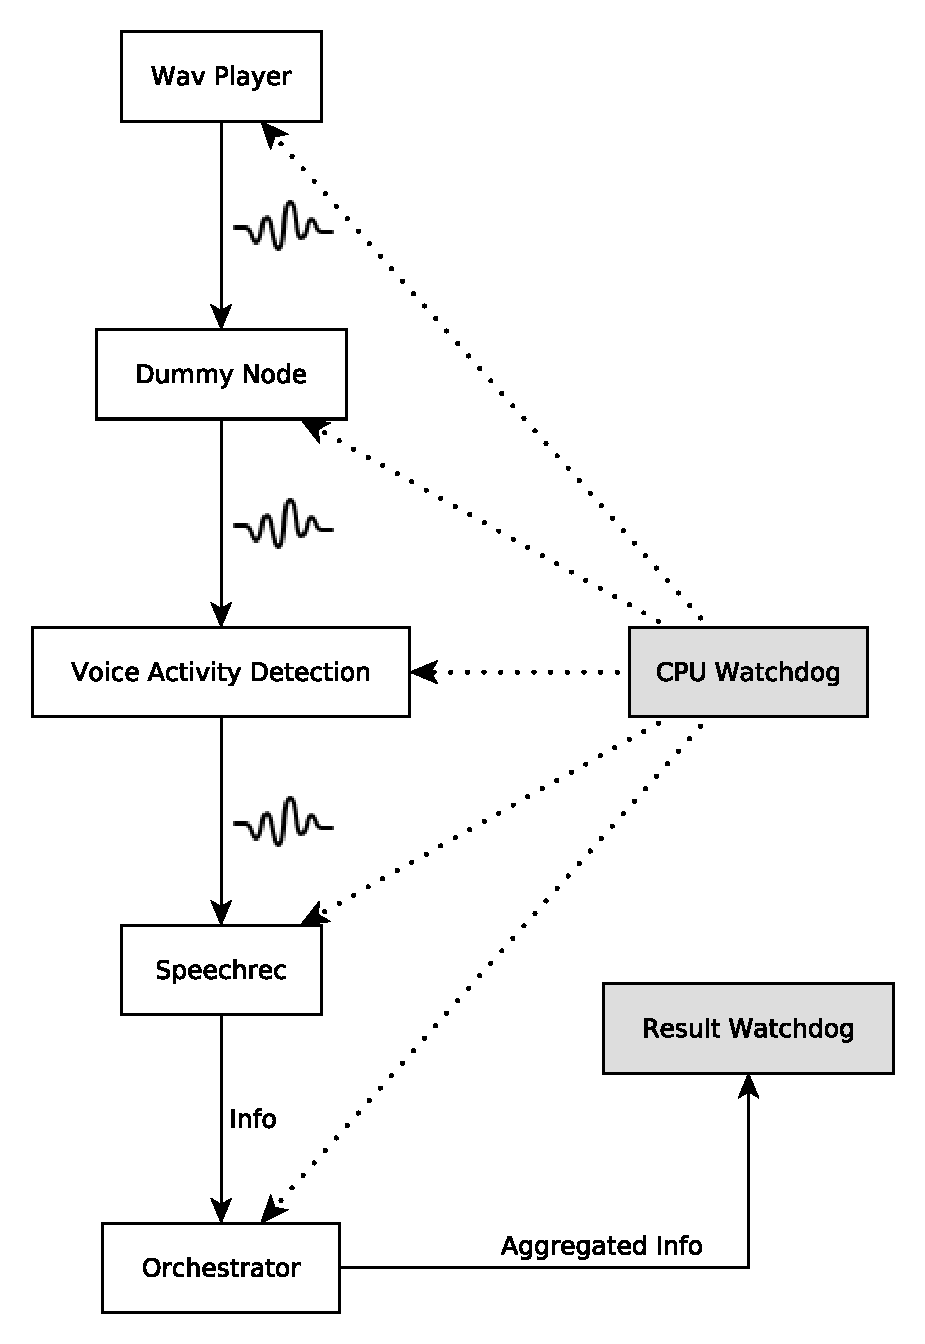
\includegraphics[width=0.5\textwidth]{diagrams/eval_pipeline_4.pdf}
	}
	
	\caption{Test scenarios for proposed pipeline}
	\label{pic:eval_p2_4_diag}
\end{figure}


\begin{figure}[ht]	
	\centering
	\subfloat[Test scenario for widened baseline of proposed pipeline]{
		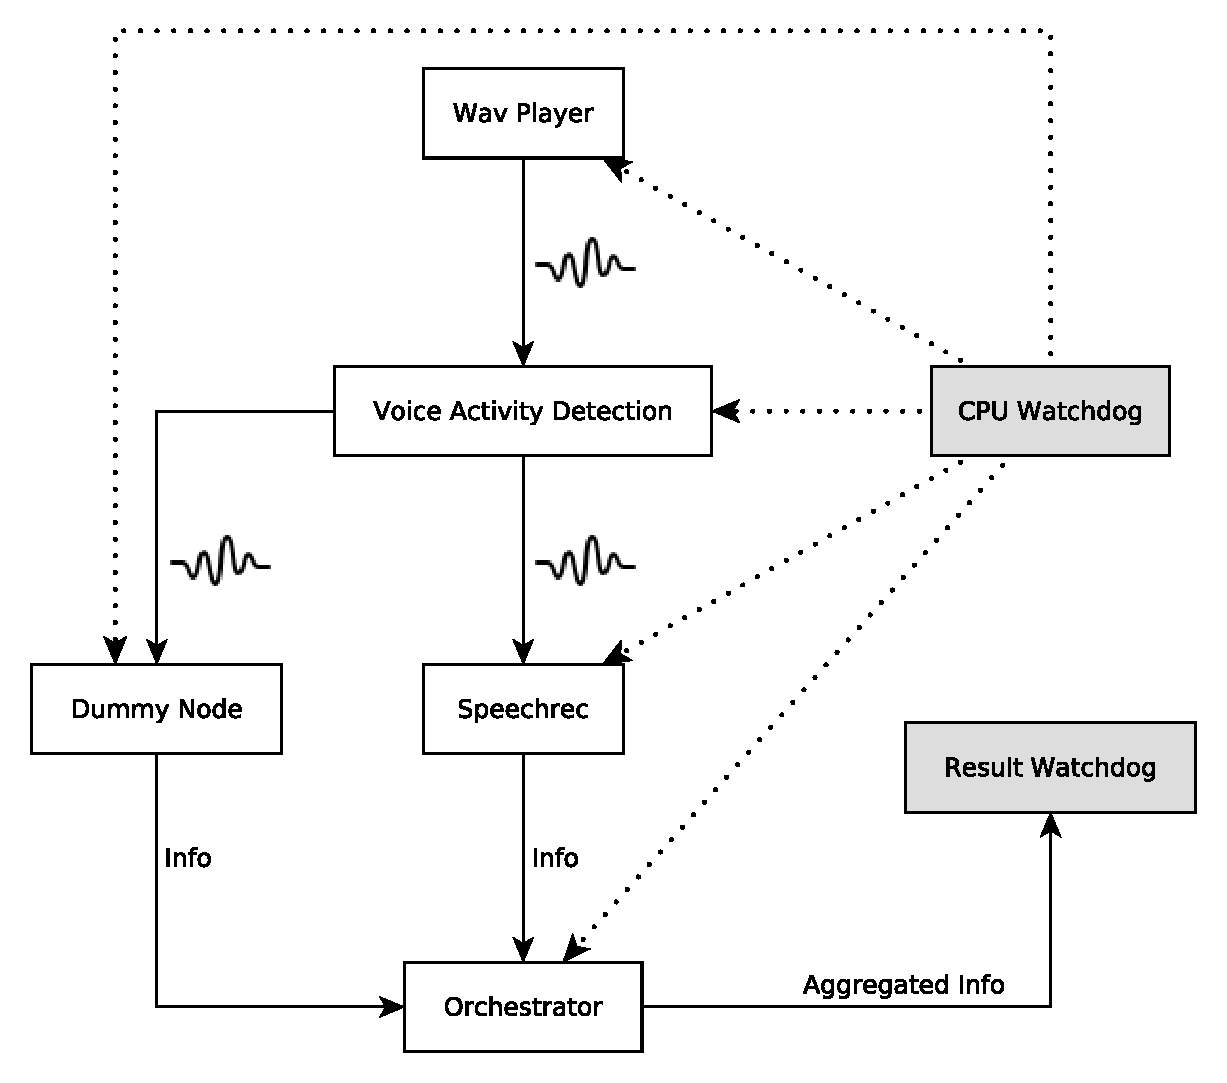
\includegraphics[width=0.5\textwidth]{diagrams/eval_pipeline_3.pdf}
	}
	\subfloat[Test scenario for elongated baseline of proposed pipeline]{
		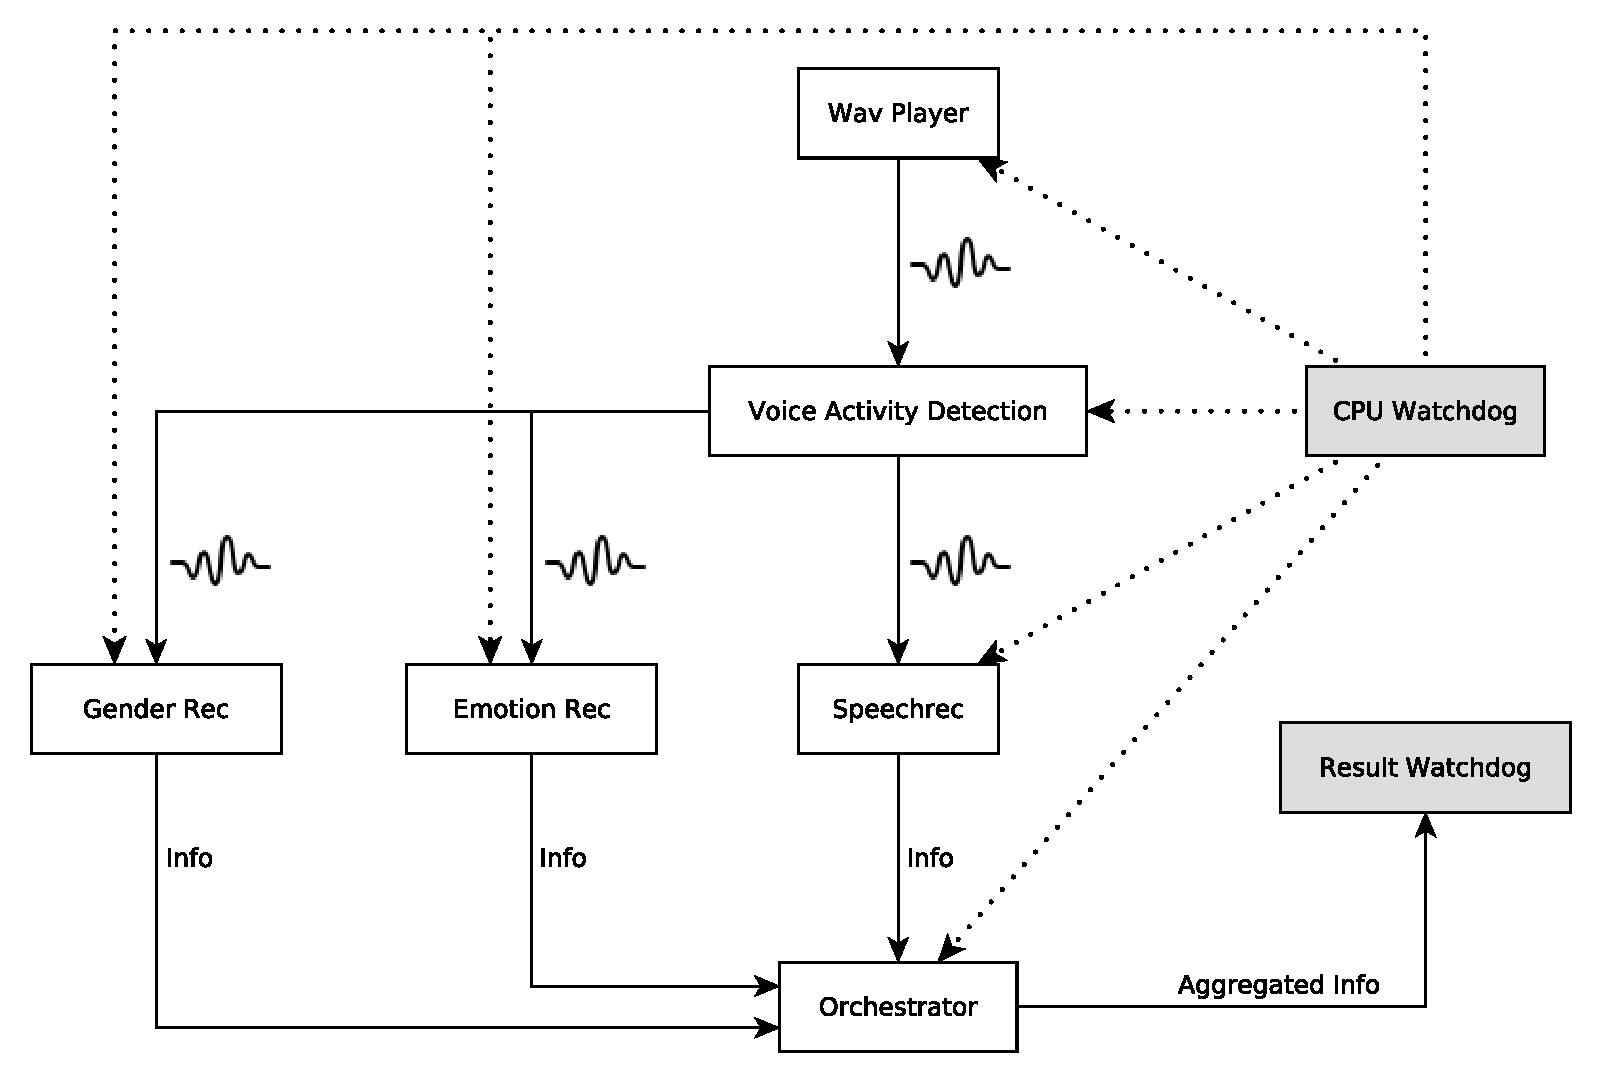
\includegraphics[width=0.5\textwidth]{diagrams/eval_pipeline_5.pdf}
	}
	
	\caption{Test scenarios for proposed pipeline}
	\label{pic:eval_p3_5_diag}
\end{figure}

\begin{figure}[ht]
	\begin{tabular}{ | l | p{0.3\textwidth} | p{0.3\textwidth} | p{0.3\textwidth} |}
		\hline
		Run & Correctly recognized sentences & Absolute time till result (in seconds) & CPU time (in CPU seconds) \\ \hline
		1 & xx.xx\% & x.xxxx & xxxx.x \\ \hline
		2 & 99.77\% & 1.0141 & 1209.3 \\ \hline
		3 & 99.65\% & 1.0899 & 1665.66 \\ \hline
		4 & 99.77\% & 1.0394 & 1399.63 \\ \hline
		5 & 99.48\% & 1.7799 & 37517.13 \\ \hline
	\end{tabular}
	\caption{Results of the pipelines in comparison}
	\label{pic:eval_dataset_results}
\end{figure}


\subsection{Existing Solution}

Goal: provide a baseline

What can be seen: 

\subsection{Baseline for proposed Pipeline}

Goal: get additional cost the pipeline itself generates against the existing solution

What can be seen: 

\subsection{Elongated baseline of proposed Pipeline}

Goal: get the overhead in time and cpu cost a single additional component does to the pipeline

What can be seen: overhead cost of adding component is rather small, especially in absolute time needed (2.5 ms), thus negligible

\subsection{Widened baseline of proposed Pipeline}

Goal: get overhead cost of a parallel component

What can be seen: 

\subsection{Realistic version of proposed Pipeline}

Goal: 

What can be seen: 
